\chapter{BERTopic}
L'avvento dei moderni \emph{LLM} ha portato ad un'evoluzione del \textbf{NLP} (Natural Language Processing) con la conseguente nascita di nuovi framework e tecniche per le analisi più disparate.
Il \emph{topic modeling} non è esente da questo fenomeno, in particolare i modelli basati su \textbf{transformers} (cioè modelli che convertono testo in embeddings dipendenti dal contesto) si sono rilevati particolarmente efficaci nell'\emph{NLP}.
\textbf{Modelli preaddestrati} sono molto utilizzati perché permettono di creare rappresentazioni \textbf{accurate} e \textbf{rappresentative} di testi, potendo fare affidamento su dataset di training molto grandi e molto diversificati.
In questo contesto BERTopic è un \textit{framework} al passo con il corrente stato dell'arte, che offre alcuni vantaggi rispetto a tecniche antecedenti, fra cui permette di catturare il \textbf{significato semantico} dei documenti (riconosce ad esempio i sinonimi). Per dataset eterogenei e rumorosi come gli annunci di lavoro, questa capacità di individuare strutture semantiche latenti rende BERTopic una scelta particolarmente vantaggiosa rispetto ai modelli tradizionali. Inoltre in BERTopic specificare il il numero di classi è \textbf{opzionale}.
Inoltre BERTopic è composto da più \textit{submodules} con funzioni diverse, il che permette un'alta personalizzazione.

\section{Funzionalità}
All'interno di Bert Topic è possibile distinguere alcune funzionalità particolarmente utili per questo progetto:
\begin{enumerate}
\item Embedding
\item Dimensionality Reduction
\item Clustering
\item CountVectorizer
\item c-TF-IDF
\end{enumerate}

BERTopic permette l'utilizzo di algoritmi diversi per ogni funzionalità, per personalizzare il proprio \emph{topic model}, ad esempio il clustering può essere effettuato da \emph{HDBSCAN} o da \emph{k-Means}.
Illustreremo ora tutti i moduli da noi usati, vedremo nello specifico la loro funzione e come la loro alterazione modifica il risultato finale.
\subsection{Embedding}
Il primo modulo è l’embedder, il cui compito è quello di trasformare i documenti testuali in rappresentazioni numeriche poi utilizzabili dagli algoritmi di machine learning.

\noindent Il testo viene innanzitutto \textbf{tokenizzato}: un token può corrispondere a una parola intera, a una sua parte oppure a una sequenza di caratteri frequente, in base alla strategia di tokenizzazione adottata.

\noindent Ciascun token è successivamente convertito in un vettore numerico, l’\textit{embedding}. Questi vettori abitano uno spazio ad alta dimensionalità in cui la vicinanza geometrica riflette la somiglianza semantica dei token: parole con significato analogo (ad esempio \textit{developer} e \textit{programmer}) finiscono in posizioni contigue.

\begin{figure}[H]
\centering
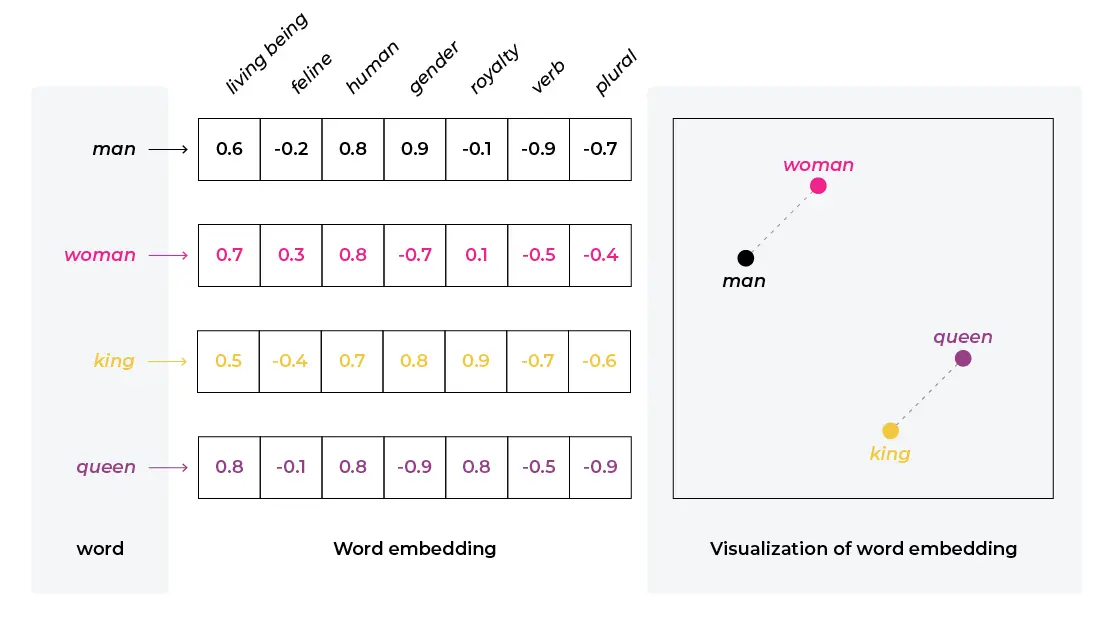
\includegraphics[width=0.6\textwidth]{BERTopic/embeddings/blog-king-queen-embeddings.jpg}
\caption{Esempio illustrativo di relazioni semantiche nello spazio degli embedding: differenze vettoriali come $E(\text{man})-E(\text{woman})$ codificano attributi latenti (qui il genere).}
\label{fig:embedding-analogy}
\end{figure}

\noindent Nella Figura~\ref{fig:embedding-analogy} si osserva come la direzione del vettore $E(\text{man})-E(\text{woman})$ (dove $E(\cdot)$ è la funzione di embedding) catturi una proprietà semantica interpretabile.

\noindent La dimensionalità di questo spazio dipende dal modello: \textit{all-mpnet-base-v2} produce vettori da 768 componenti, mentre modelli di grandi dimensioni come GPT-3 arrivano a 12\,288 dimensioni. Negli embedder moderni (ad esempio quelli basati su Transformer), ad esempio \textit{Sentence-BERT} (SBERT), MPNet o GPT, ogni token viene inoltre rappresentato \textit{in funzione del contesto} in cui compare. Di conseguenza la parola “bank” avrà embedding diversi se usata in “river bank” oppure in “investment bank”.

\noindent A partire dagli embedding dei token è possibile costruire \textit{sentence embeddings} che sintetizzano la struttura sintattico-semantica di un paragrafo. SBERT, in particolare, applica un meccanismo di pooling (tipicamente mean o max pooling)\footnote{\url{https://sbert.net/docs/package_reference/sentence_transformer/models.html}} alle rappresentazioni prodotte dal Transformer, ottenendo un unico vettore che compendia l’informazione distribuita sull’intera frase.

\noindent L’uso di \textit{sentence embeddings} consente di calcolare \textbf{distanze semantiche tra documenti} con misure come cosine similarity o euclidean distance, rendendoli ideali per compiti quali \textit{clustering} e \textit{topic discovery}.
\subsection{Dimensionality Reduction}
I vettori generati dall'embedder hanno dimensione alta, a prescindere dal modello che si sceglie e ciò potrebbe rendere difficile il \emph{clustering}. Per questo è importante introdurre nella pipeline un algoritmo di riduzione della dimensione.
L'idea di questi algoritmi è quella di ridurre la dimensione di un insieme di vettori preservandone la \textbf{struttura topologica locale}.
Di default BERTopic usa \textbf{UMAP}\footnote{\url{https://maartengr.github.io/BERTopic/getting_started/dim_reduction/dim_reduction.html}} per questo compito poiché \emph{preserva sia la struttura locale, che quella globale degli spazi ad alte dimensioni}.
UMAP lavora costruendo un \textit{grafo fuzzy locale}: ogni punto viene connesso ai suoi \texttt{n\_neighbors} più vicini e la connessione è pesata in base alla distanza. Questo grafo rappresenta la topologia locale dello spazio originale.
UMAP cerca poi una rappresentazione a bassa dimensione che minimizzi la differenza tra il grafo originale e il grafo proiettato.

L'obiettivo è mantenere la densità e la vicinanza dei punti simili, consentendo allo stesso tempo di contrarre regioni sparse.
Questo bilanciamento consente di preservare la struttura locale pur comprimendo lo spazio globale.
Vediamo più nel dettaglio questi punti.
\subsubsection{Fuzzy simplicial complex}
Per costruire il grafo iniziale ad alta dimensionalità, \textbf{UMAP} crea una struttura chiamata \textit{fuzzy simplicial complex}. In pratica, si tratta di una rappresentazione di un grafo pesato, in cui i pesi degli archi rappresentano la \textbf{probabilità che due punti siano connessi}.

Per determinare la connessione tra due punti, UMAP\footnote{\url{https://pair-code.github.io/understanding-umap/}} estende un \textbf{raggio locale} a partire da ciascun punto e collega i punti quando i rispettivi raggi si sovrappongono. La scelta di questo raggio è cruciale:
Se è troppo piccolo, il risultato sarà un insieme di \textbf{piccoli cluster isolati};
se è troppo grande, tutti i punti finiranno per essere \textbf{collegati tra loro}, perdendo così la struttura locale.

UMAP risolve questo problema scegliendo un raggio locale \textbf{adattivo}, basato sulla distanza rispetto al $k$-esimo vicino più prossimo di ciascun punto. Successivamente, il grafo viene reso ``sfumato'' (\textit{fuzzy}) diminuendo la probabilità di connessione man mano che la distanza aumenta.

Infine, imponendo che ogni punto sia connesso almeno al proprio vicino più prossimo, UMAP garantisce un equilibrio tra la \textbf{preservazione della struttura locale} e la \textbf{coerenza della struttura globale}.
\begin{figure}[H]
\centering
\includegraphics[width=0.75\textwidth]{img/BERTopic/umap/UMAP\_projection.png}
\caption{Proiezione UMAP nel piano bidimensionale. Dopo l'intersezione con il primo \emph{neighbour}, il cerchio diventa \emph{sfumato}, riducendo il peso della connessione.\protect\footnotemark}
\label{fig:umap-projection}
\end{figure}
\footnotetext{\url{https://pair-code.github.io/understanding-umap/}}
\subsubsection{Parametri}
I due parametri più importanti di UMAP sono \texttt{n\_neighbors} e \texttt{min\_dist}, poiché regolano l'equilibrio tra struttura \textit{locale} e \textit{globale} nella proiezione finale.\footnote{\url{https://pair-code.github.io/understanding-umap/}}

\paragraph{\texttt{n\_neighbors}.} Determina il numero di vicini utilizzato per costruire il grafo fuzzy iniziale. Valori bassi enfatizzano le relazioni locali, isolando micro-strutture anche molto sottili; valori alti favoriscono invece la coerenza complessiva, preservando maggiormente la geometria globale dell'insieme di punti.
Per visualizzare l'effetto di \texttt{n\_neighbors} consideriamo la proiezione bidimensionale di un modello 3D campionato con 50\,000 punti. Le immagini mostrano come la struttura globale emerga gradualmente all'aumentare del numero di vicini, mentre i dettagli fini sono preservati soltanto per valori più bassi.

\begin{figure}[H]
\centering
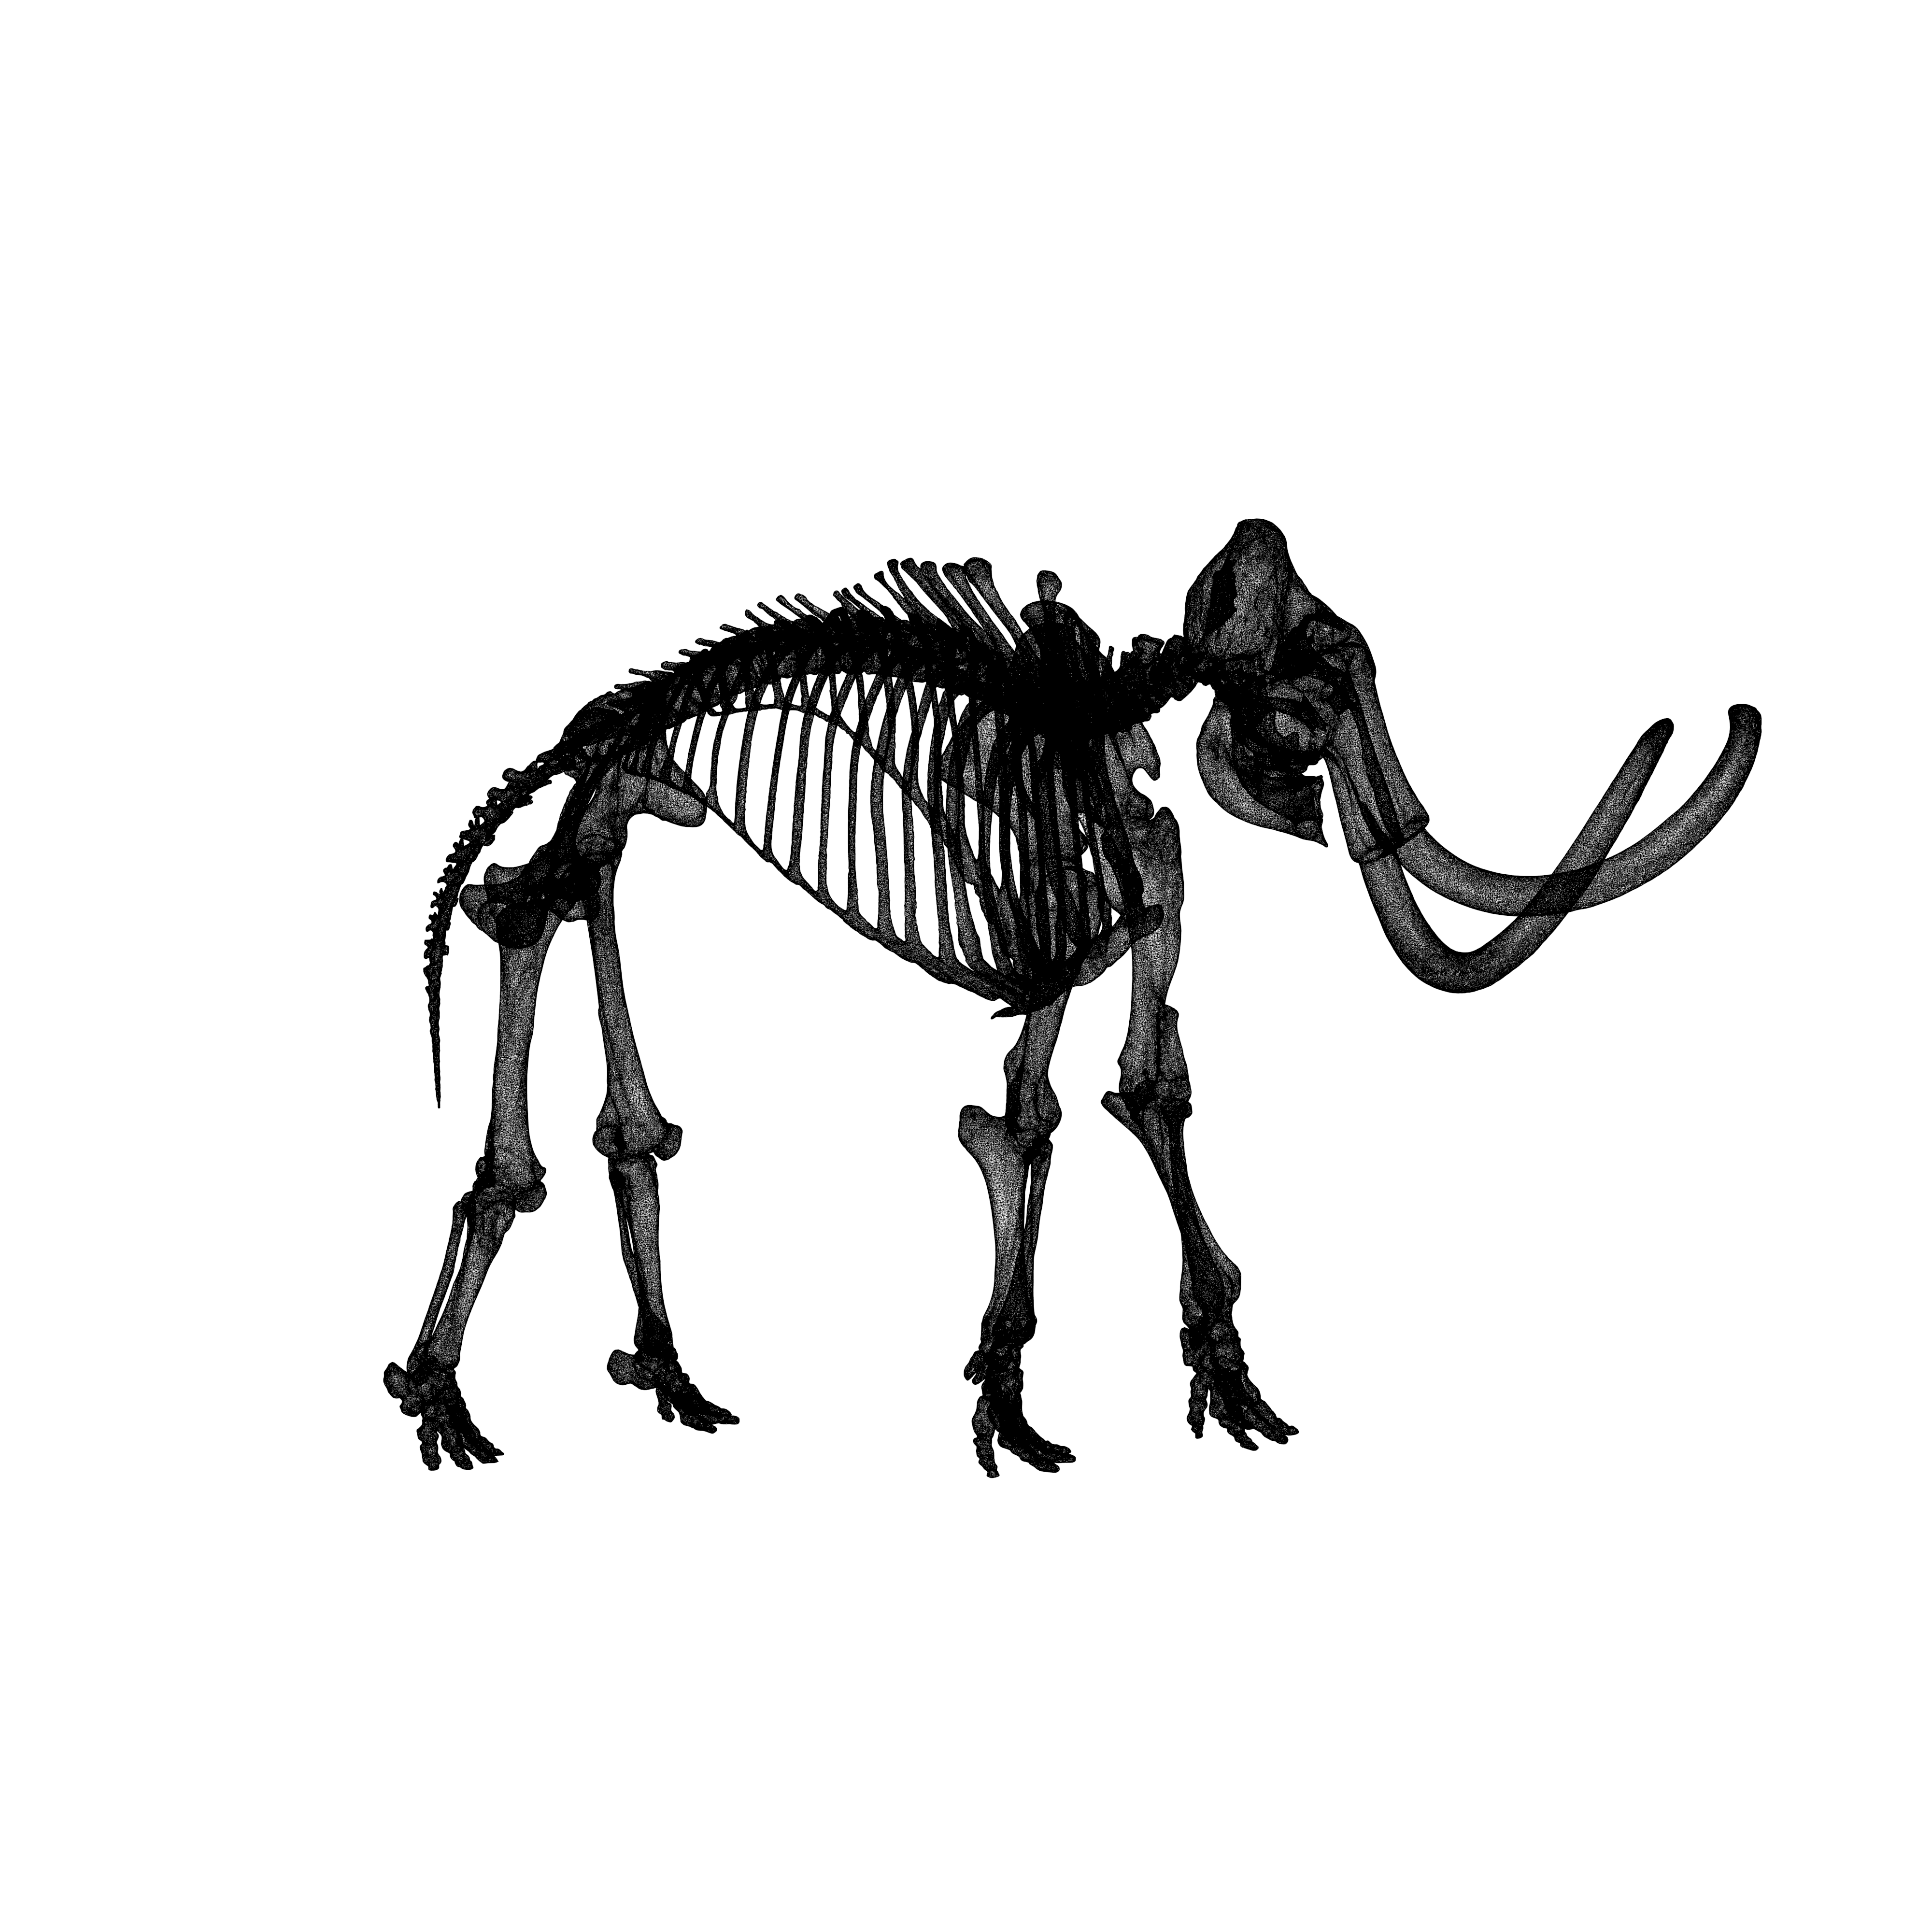
\includegraphics[width=0.5\textwidth]{BERTopic/umap/mammoth_render.png}

\begin{subfigure}{0.32\textwidth}
    \centering
    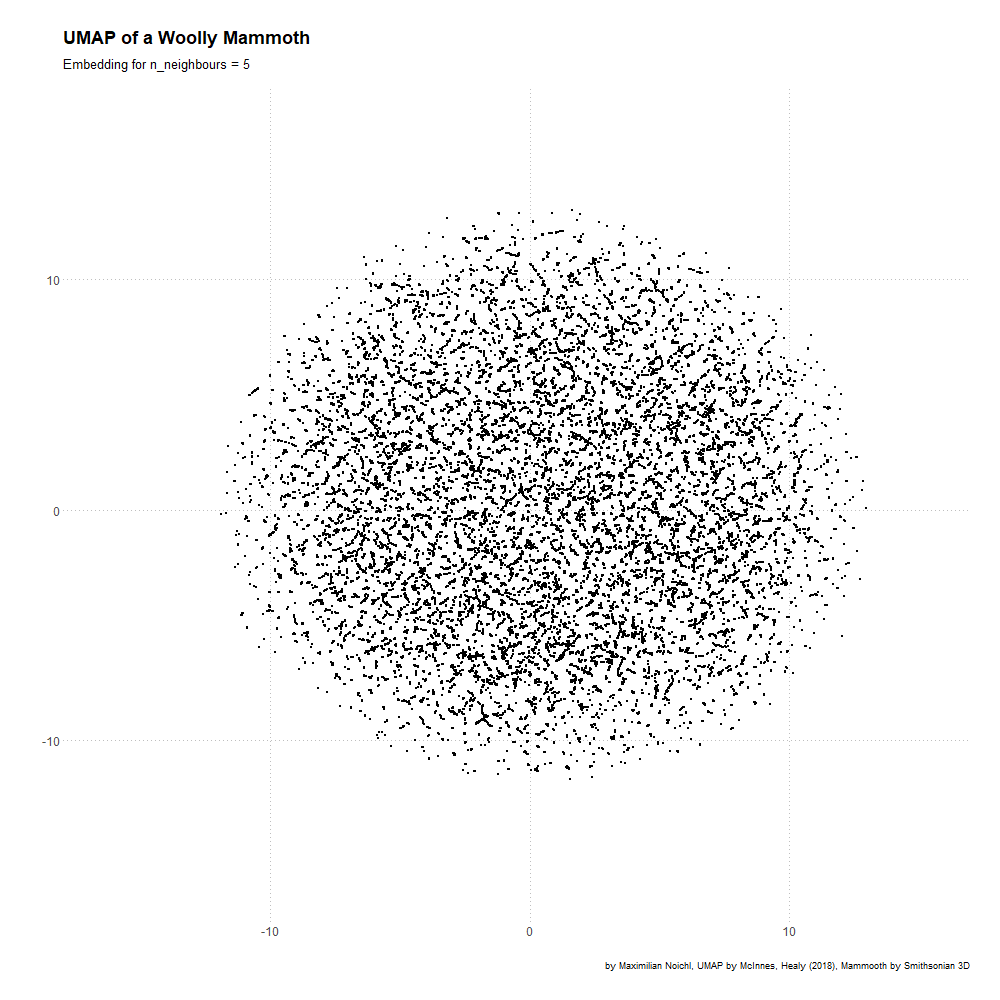
\includegraphics[width=\textwidth]{BERTopic/umap/n_neighbours5.png}
    \caption{$n\_neighbors = 5$}
\end{subfigure}\hfill
\begin{subfigure}{0.32\textwidth}
    \centering
    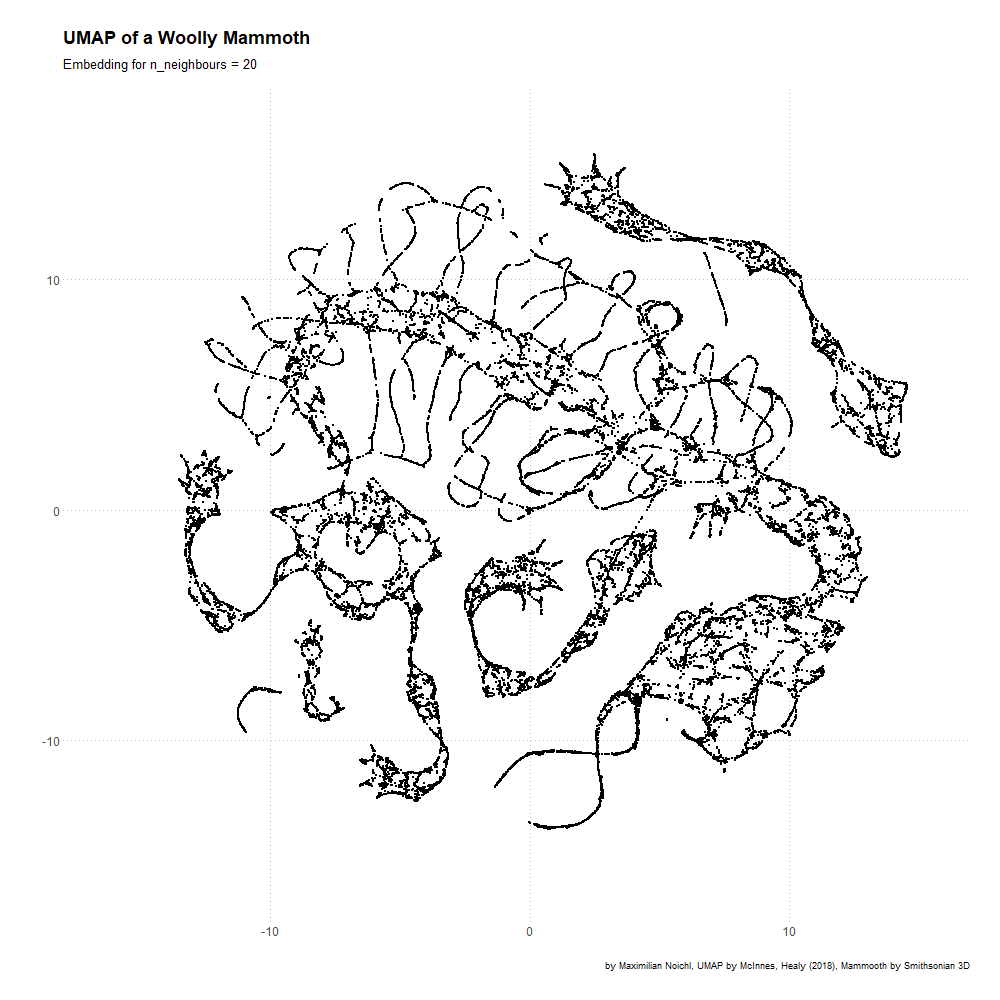
\includegraphics[width=\textwidth]{BERTopic/umap/n_neighbours20.png}
    \caption{$n\_neighbors = 20$}
\end{subfigure}\hfill
\begin{subfigure}{0.32\textwidth}
    \centering
    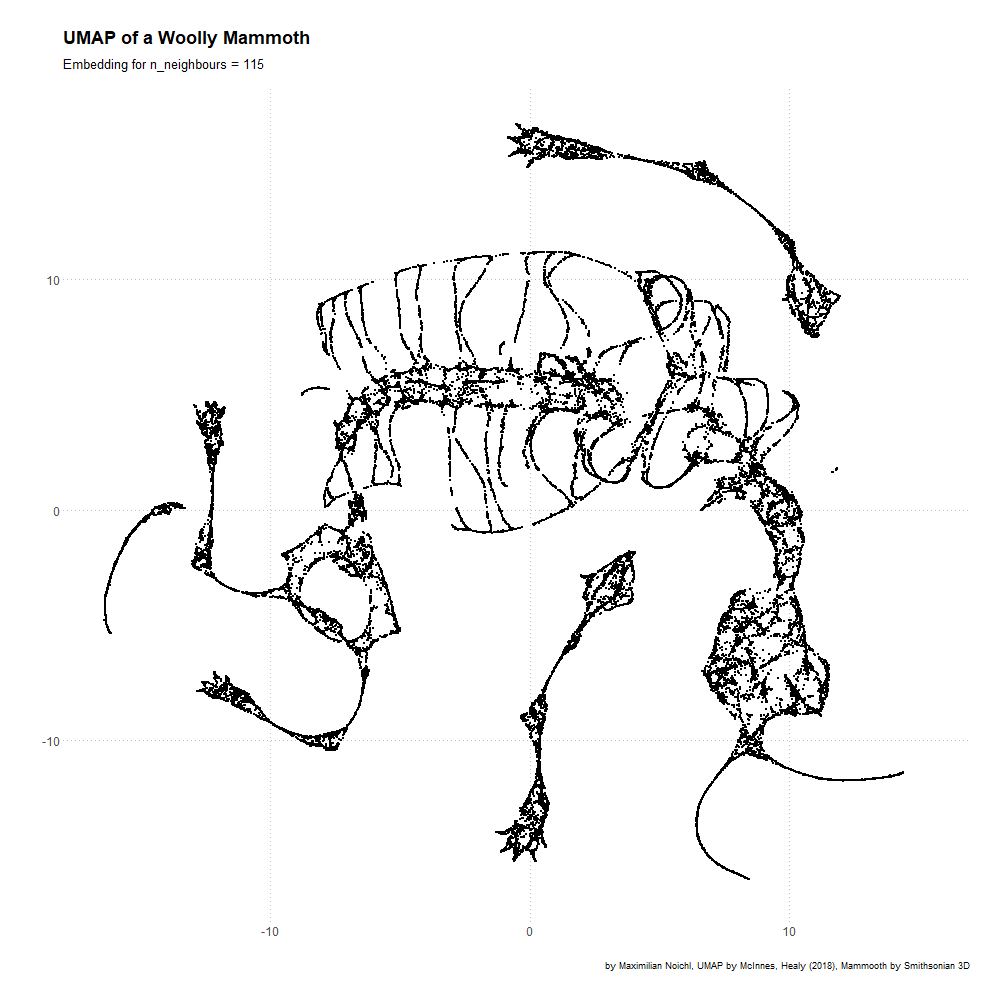
\includegraphics[width=\textwidth]{BERTopic/umap/n_neighbours115.png}
    \caption{$n\_neighbors = 115$}
\end{subfigure}
\caption{Proiezione UMAP di un modello 3D con 50\,000 punti in un piano 2D. Fonti: \href{https://3d.si.edu/object/3d/mammuthus-primigenius-blumbach:341c96cd-f967-4540-8ed1-d3fc56d31f12}{Smithsonian 3D Digitization Program} e \href{https://www.maxnoichl.eu/projects/mammoth/}{Max Noichl}.}
\label{fig:umap-mammoth}
\end{figure}Si osservi come per valori ridotti di \texttt{n\_neighbors} la proiezione UMAP mantenga dettagli locali (curve delle zanne o delle zampe), ma perda la forma complessiva del mammut; all'aumentare del parametro la sagoma globale diventa riconoscibile, a scapito delle piccole variazioni geometriche.
\paragraph{\texttt{min\_dist}} controlla la densità minima consentita nella proiezione a bassa dimensione. Un valore vicino a zero permette ai punti di collassare in regioni molto dense, mettendo in risalto cluster ben separati; aumentando il parametro, UMAP distribuisce i punti con maggiore uniformità, sacrificando la compattezza dei gruppi a favore di una rappresentazione più omogenea. La Figura~\ref{fig:umap-min-dist} mostra come diverse configurazioni di \texttt{min\_dist} modifichino la distribuzione dei punti: valori estremamente bassi generano isole molto concentrate, mentre impostazioni più elevate distendono l'intero spazio proiettato.
\begin{figure}[H]
\centering

\begin{subfigure}{0.32\textwidth}
    \centering
    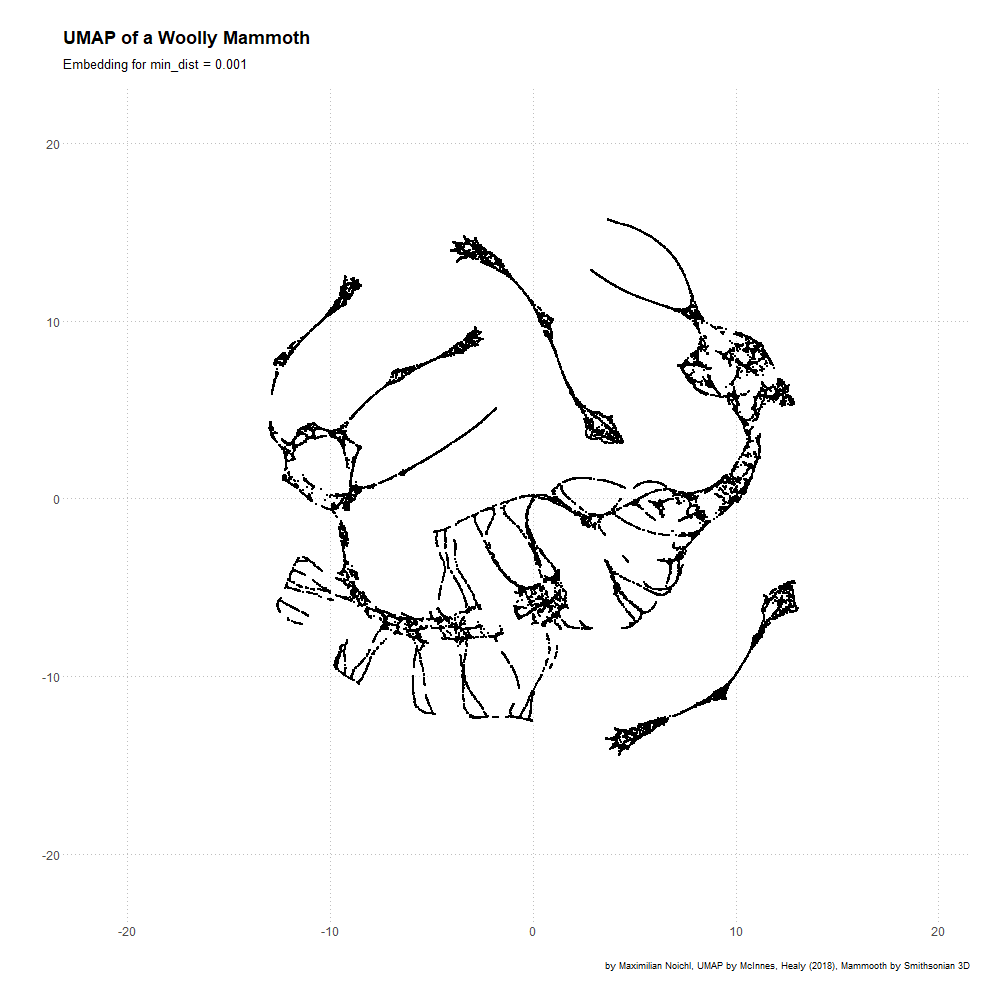
\includegraphics[width=\textwidth]{BERTopic/umap/min_dist_001.png}
    \caption{$min\_dist = 0.01$}
\end{subfigure}\hfill
\begin{subfigure}{0.32\textwidth}
    \centering
    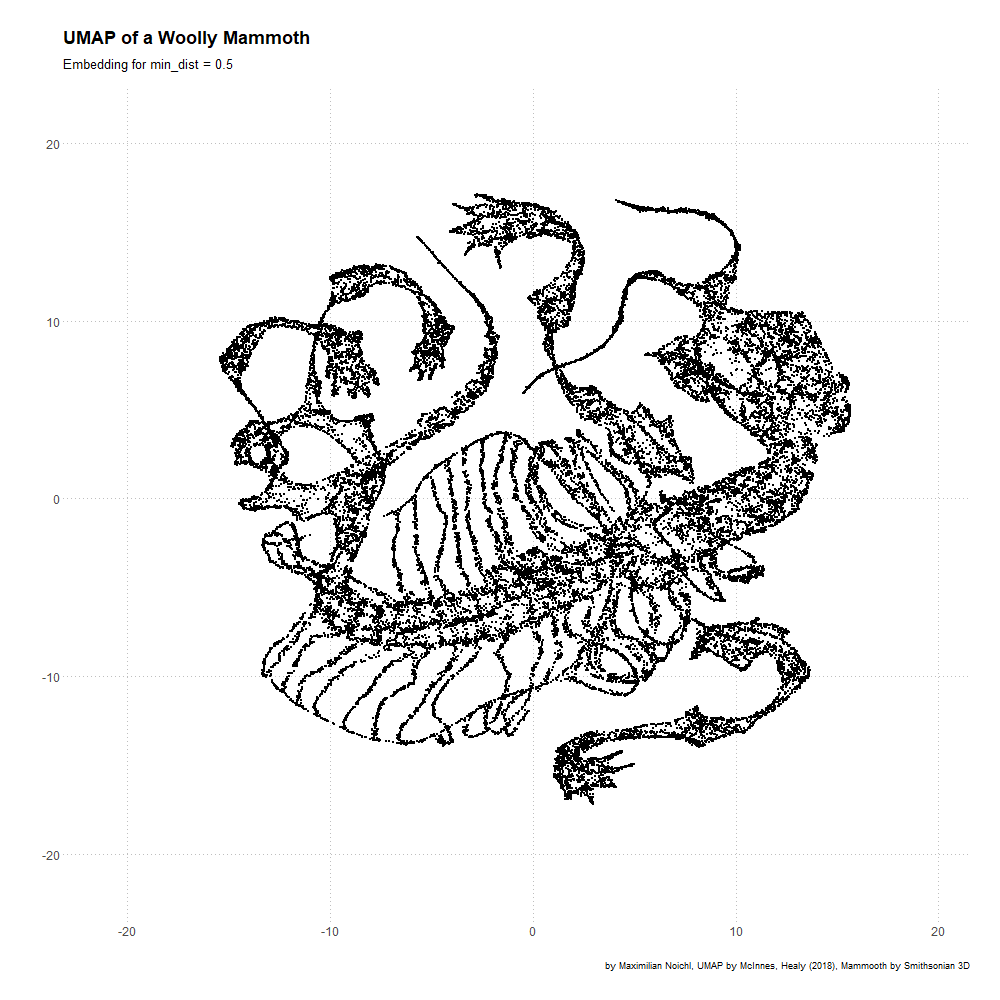
\includegraphics[width=\textwidth]{BERTopic/umap/m_dist_5.png}
    \caption{$min\_dist = 0.5$}
\end{subfigure}\hfill
\begin{subfigure}{0.32\textwidth}
    \centering
    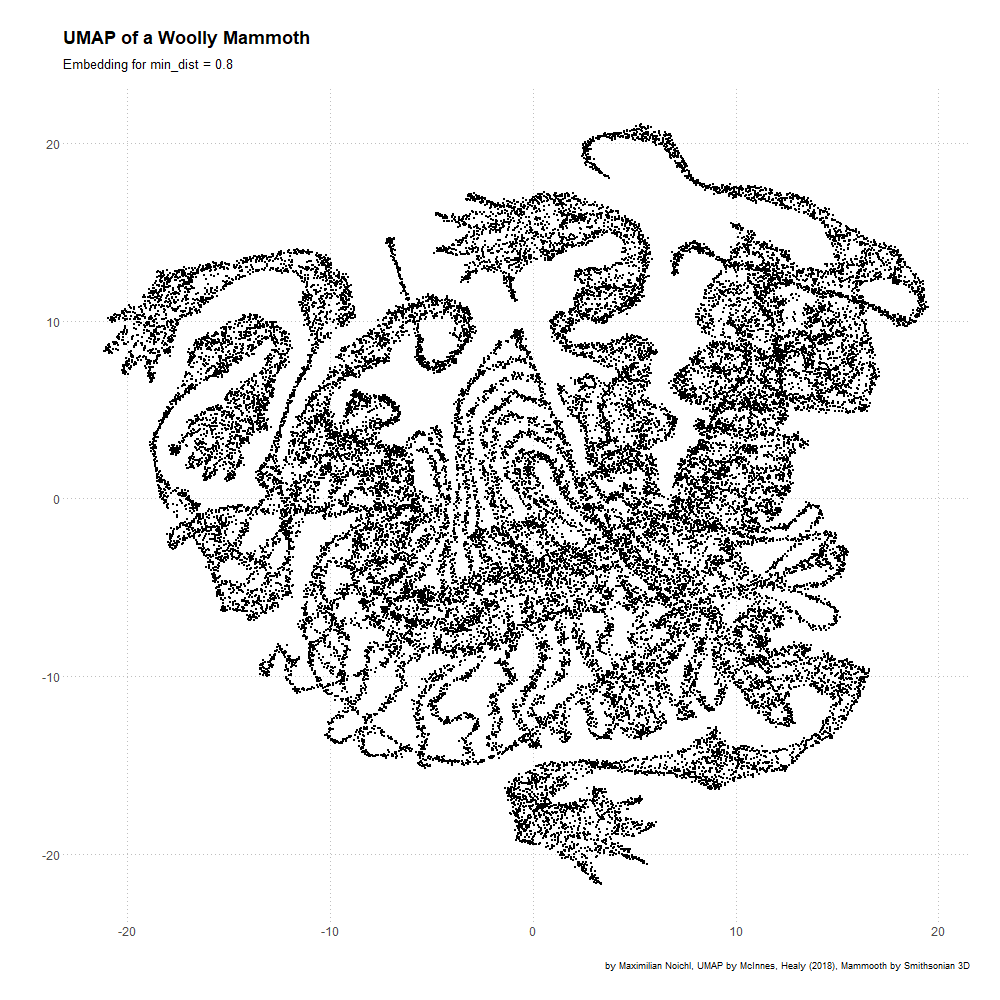
\includegraphics[width=\textwidth]{BERTopic/umap/m_dist_8.png}
    \caption{$min\_dist = 0.8$}
\end{subfigure}
\caption{Effetto di \texttt{min\_dist} sulla proiezione UMAP del modello 3D da 50\,000 punti. Fonti: \href{https://3d.si.edu/object/3d/mammuthus-primigenius-blumbach:341c96cd-f967-4540-8ed1-d3fc56d31f12}{Smithsonian 3D Digitization Program} e \href{https://www.maxnoichl.eu/projects/mammoth/}{Max Noichl}.}
\label{fig:umap-min-dist}
\end{figure}
\subsection{Clustering}
\noindent Dopo aver ridotto la dimensione dell'input, dobbiamo creare dei \textit{cluster} di embedding simili da cui estrarremo i topic.

\noindent Il modello che consiglia BERTopic\footnote{\url{https://maartengr.github.io/BERTopic/getting_started/clustering/clustering.html}} è \textit{HDBSCAN}, un algoritmo di clustering basato su densità, in modo da identificare cluster a densità variabile senza dover fissare un singolo parametro di soglia (a differenza di \textit{DBSCAN}).

\noindent Il \textit{clustering} viene ottenuto passando per 5 fasi\footnote{\url{https://hdbscan.readthedocs.io/en/latest/how_hdbscan_works.html}}:
\begin{enumerate}
    \item Trasformazione dello spazio basata sulla densità
    \item Minimum spanning tree del grafo pesato delle distanze
    \item Costruzione della gerarchia di aggregazione dei punti
    \item Condensazione della gerarchia in base a \texttt{min\_cluster\_size}
    \item Estrazione dei cluster dall'albero condensato
\end{enumerate}

Vediamo i passaggi più nel dettaglio con l'ausilio di un esempio grafico. In Figura~\ref{fig:hdbscan-points} è mostrato l'insieme di punti su cui applicheremo HDBSCAN.
\begin{figure}[H]
\centering
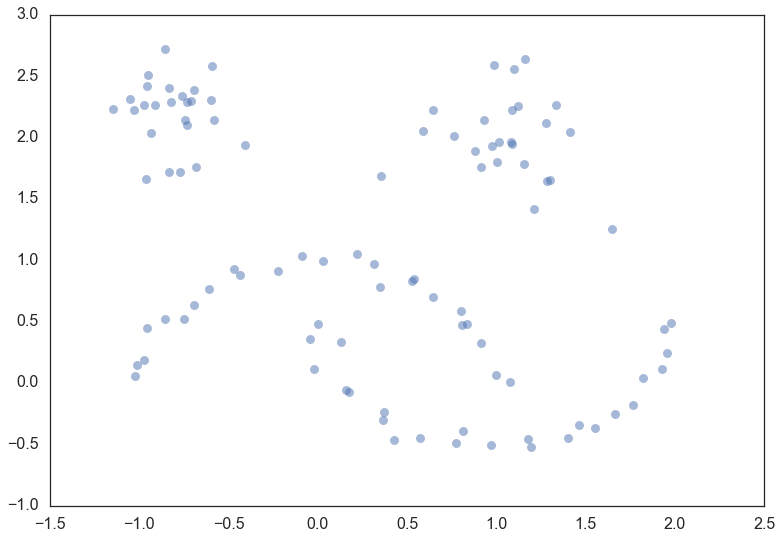
\includegraphics[width=0.65\textwidth]{BERTopic/hdbscan/hdbscan_points.png}
\caption{Dataset iniziale \textit{ad hoc} generato per testare HDBSCAN}
\label{fig:hdbscan-points}
\end{figure}
\subsubsection*{1. Trasformazione dello spazio in funzione della densità}

Il primo passo dell'algoritmo HDBSCAN consiste nel \textit{trasformare lo spazio dei dati} in modo che rifletta non solo la distanza geometrica tra i punti, ma anche la \textbf{densità locale} delle regioni in cui essi si trovano. 
Questo passaggio consente di adattare la nozione di distanza alle caratteristiche strutturali del dataset, migliorando la robustezza rispetto a variazioni di scala e rumore.

Per ogni punto \( x_i \) viene calcolata la \textbf{core distance}, definita come la distanza dal suo \( k\)-esimo vicino più prossimo, dove \( k = \text{min\_samples} \). 
Essa rappresenta una stima della densità locale: valori piccoli indicano aree dense, mentre valori grandi indicano zone più sparse o isolate.

Successivamente, la distanza tra due punti \( a \) e \( b \) viene ridefinita come \textbf{mutual reachability distance}, che tiene conto delle rispettive densità locali:

\[
d_{\text{mreach}}(a,b) = \max \big( \text{core\_dist}(a),\ \text{core\_dist}(b),\ d(a,b) \big)
\]
dove $d(a,b)$ è la distanza originale tra $a$ e $b$. Usando questa distanza, i punti densi rimangono alla loro distanza originale, mentre quelli rarefatti vengono allontanati, ciò rende l'algoritmo \textbf{robusto al rumore}.
\subsubsection*{2. Costruzione del \textit{Minimum Spanning Tree} (MST)}

Dopo la trasformazione dello spazio in funzione della densità locale, HDBSCAN costruisce un grafo completamente connesso in cui ogni punto rappresenta un nodo e ogni arco tra due punti è pesato in base alla \textit{mutual reachability distance} calcolata nel passo precedente. 
Questo grafo descrive la struttura di connettività del dataset, tenendo conto sia della distanza geometrica sia della densità locale delle regioni considerate.

A partire da tale grafo, viene poi calcolato il \textbf{Minimum Spanning Tree} (MST), ossia l'albero di connessioni che collega tutti i punti minimizzando la somma complessiva dei pesi degli archi. 
Il MST conserva quindi solo le connessioni essenziali per mantenere la connettività globale, eliminando i collegamenti ridondanti e le connessioni tra regioni scarsamente dense.

Questo passaggio ha due obiettivi principali:
\begin{itemize}
    \item \textbf{Semplificare la struttura dei dati}, riducendo la complessità del grafo e mantenendo una rappresentazione compatta della topologia di densità;
    \item \textbf{Preparare la costruzione della gerarchia dei cluster}, poiché nei passi successivi gli archi del MST verranno rimossi in ordine crescente di distanza per individuare i gruppi di punti che restano connessi, ossia i futuri cluster.
\end{itemize}

il Minimum Spanning Tree dunque connette i punti più vicini secondo la loro densità locale e costituisce la base per la costruzione della gerarchia dei cluster nel passo successivo.

\begin{figure}[H]
\centering
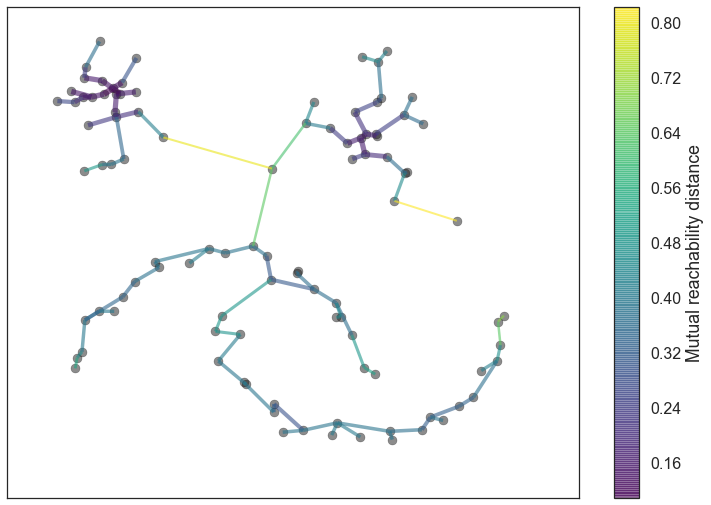
\includegraphics[width=0.65\textwidth]{BERTopic/hdbscan/hdbscan_MST.png}
\caption{Minimum Spanning Tree costruito sulle distanze di mutual reachability: gli archi a peso minore collegano regioni dense e fungono da base per la gerarchia.}
\label{fig:hdbscan-mst}
\end{figure}

\subsubsection*{3. Costruzione della gerarchia dei cluster}

A partire dal \textit{Minimum Spanning Tree} costruito nel passo precedente, HDBSCAN procede alla \textbf{costruzione di una gerarchia di cluster} basata sulle componenti connesse del grafo. 
Questo processo consiste nel rimuovere progressivamente gli archi del MST in ordine crescente di peso, ovvero dalla connessione più ``debole'' (distanza maggiore) a quella più ``forte'' (distanza minore).

Man mano che gli archi vengono rimossi, il grafo si frammenta in un numero crescente di componenti connesse. 
Ogni componente risultante viene interpretata come un potenziale cluster a un determinato livello di densità. 
In questo modo, HDBSCAN genera una \textit{gerarchia di densità} in cui i cluster ``nascono'' e ``muoiono'' al variare della soglia di distanza, descrivendo come la struttura dei dati cambia al modificarsi del livello di densità considerato.

Il risultato di questa fase è un albero gerarchico che rappresenta la relazione di inclusione tra cluster: 
le radici corrispondono ai cluster più generali (densità minore), mentre i rami e le foglie rappresentano i cluster più specifici e densi. 
Questa rappresentazione gerarchica è fondamentale per le fasi successive, poiché consente di identificare in modo naturale i livelli di densità più stabili e significativi all'interno del dataset.

\begin{figure}[H]
\centering
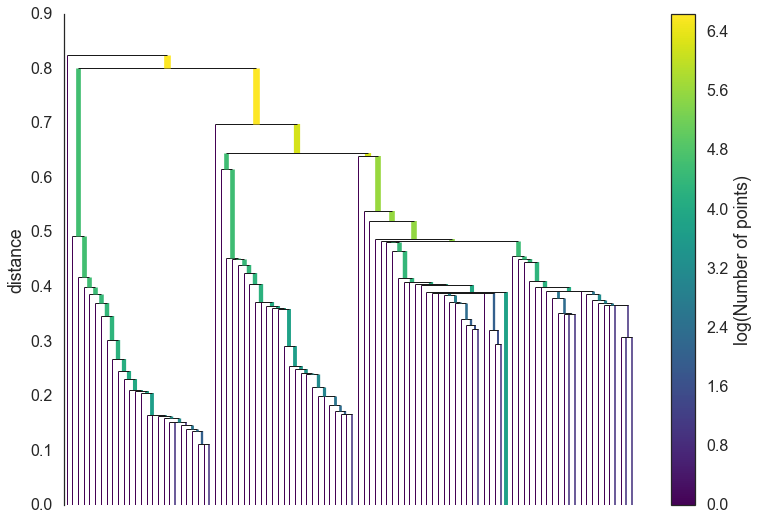
\includegraphics[width=0.65\textwidth]{BERTopic/hdbscan/hdbscan_cluster_hierarchy.png}
\caption{Esempio di gerarchia dei cluster derivata dalla rimozione progressiva degli archi del MST: i nodi mostrano come i gruppi nascano e si separino a densità crescenti.}
\label{fig:hdbscan-cluster-hierarchy}
\end{figure}

\subsubsection*{4. Condensazione della gerarchia dei cluster}

Una volta costruita la gerarchia completa delle componenti connesse, HDBSCAN applica un processo di \textbf{condensazione} basato sul parametro \texttt{min\_cluster\_size}. 
L'obiettivo è semplificare la struttura gerarchica, eliminando i rami instabili e i cluster di dimensioni troppo ridotte per essere considerati significativi.

Durante questa fase, la gerarchia dei cluster viene attraversata e vengono mantenuti soltanto quei gruppi che rispettano la dimensione minima richiesta. 
I cluster che non raggiungono la soglia stabilita vengono rimossi oppure fusi con componenti più grandi a densità simile, producendo una rappresentazione compatta e più interpretabile della struttura dei dati.

Il risultato di questa operazione è un \textit{condensed tree}, ossia un albero di condensazione in cui ogni nodo rappresenta un cluster potenzialmente stabile e ogni arco riflette una relazione di inclusione o fusione tra cluster. 
Questo passaggio riduce notevolmente la complessità della gerarchia originale, preservando solo le regioni dello spazio che presentano un'evidente coesione interna e scartando i gruppi effimeri o rumorosi.

La condensazione costituisce quindi la base per la successiva selezione dei cluster più stabili, che rappresentano le strutture di densità realmente persistenti all'interno del dataset.

\begin{figure}[H]
\centering
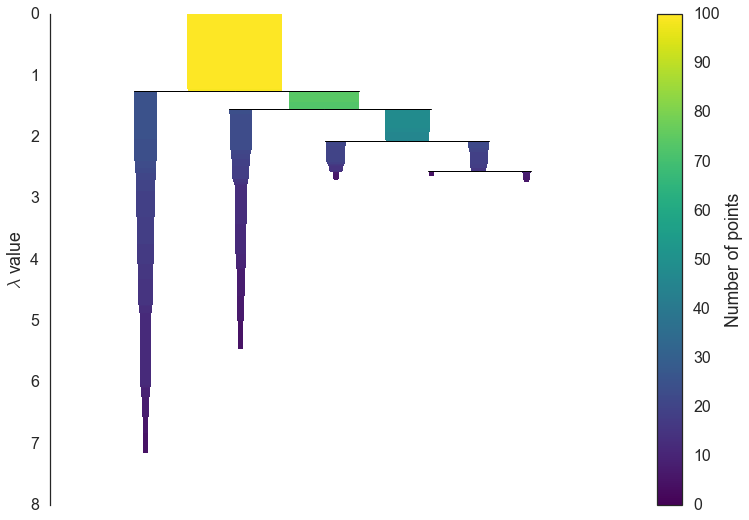
\includegraphics[width=0.65\textwidth]{BERTopic/hdbscan/hdbscan_condensed.png}
\caption{Albero condensato generato applicando \texttt{min\_cluster\_size}: vengono eliminati i rami instabili e restano solo i cluster con sufficiente supporto.}
\label{fig:hdbscan-condensed}
\end{figure}

\subsubsection*{5. Estrazione dei cluster stabili dalla struttura condensata}

Dopo aver ottenuto l'albero di condensazione, HDBSCAN seleziona i \textbf{cluster più stabili} in base alla loro persistenza lungo i diversi livelli di densità. 
Ogni cluster nella struttura condensata è caratterizzato da un intervallo di esistenza: esso ``nasce'' quando si separa da un cluster padre e ``muore'' quando, aumentando la soglia di densità, si frammenta o scompare.

Per ciascun cluster, HDBSCAN calcola una misura di \textbf{stabilità} che quantifica la sua persistenza all'interno della gerarchia. 
Durante questa fase, vengono mantenuti soltanto i cluster con una stabilità elevata, mentre i punti appartenenti a regioni meno dense o a cluster transitori vengono etichettati come \textit{rumore} (label~$-1$). 
Questo approccio consente di identificare automaticamente le strutture di densità più consistenti, senza richiedere la specifica del numero di cluster a priori.

\begin{figure}[H]
\centering
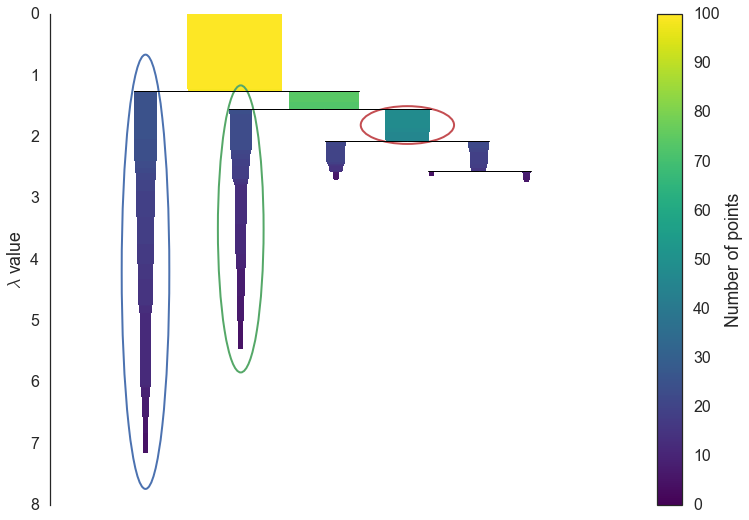
\includegraphics[width=0.65\textwidth]{BERTopic/hdbscan/hdbsca_clusters.png}
\caption{Cluster finali selezionati in base alla stabilità: i colori identificano le componenti persistenti, mentre i punti grigi rappresentano il rumore (label $-1$).}
\label{fig:hdbscan-final-clusters}
\end{figure}

\subsection{CountVectorizer}
Nel topic modeling, dopo la creazione dei topic, si cerca una \textbf{rappresentazione} che descriva i topic in termini lessicali.

Il \texttt{CountVectorizer} rappresenta il primo passo per collegare la rappresentazione semantica dei documenti, ottenuta tramite gli \textit{embeddings}, a una rappresentazione lessicale interpretabile. 
Il suo compito è quello di trasformare un insieme di testi in una matrice numerica in cui ogni riga rappresenta un documento e ogni colonna un termine del vocabolario; ciascun elemento \( M_{ij} \) indica quante volte il termine \( j \) compare nel documento \( i \).

In questo modo, il \texttt{CountVectorizer} costituisce il ponte tra la rappresentazione numerica continua degli \textit{embeddings} e la rappresentazione simbolica necessaria per calcolare le statistiche di c-TF-IDF, che servono a identificare le parole più rappresentative di ciascun topic.
\subsection{c-TF-IDF}
\noindent Come descritto nella documentazione ufficiale\footnote{\url{https://maartengr.github.io/BERTopic/api/ctfidf.html}}, il c-TF-IDF può essere visto come l’adattamento della formula TF-IDF a un contesto multi-classe: tutti i documenti di una stessa classe vengono concatenati in un unico documento, da cui si calcola la frequenza dei termini \(x\). Questa frequenza viene normalizzata con norma L1 e costituisce la \textbf{term frequency}.

Per un termine \( x \) appartenente alla classe \( c \), il peso c-TF-IDF è definito come:

\[
W_{x,c} = \left\| \mathrm{tf}_{x,c} \right\| \times 
\log \!\left( 1 + \frac{A}{f_x} \right)
\]

dove:
\begin{itemize}
    \item \( W_{x, c} \) è il peso del termine \( x\) nella classe \( c \);
    \item \( \mathrm{tf}_{x,c} \) è la frequenza del termine \( x \) nella classe \( c \);
    \item \( f_x \) è la frequenza totale del termine \( x \) considerando tutte le classi;
    \item \( A \) rappresenta il numero medio di parole per classe. 
\end{itemize}
Il termine \( \left\| \mathrm{tf}_{x,c} \right\| \) indica la normalizzazione della frequenza all'interno del topic, mentre il fattore 
\(\log \!\left( 1 + \tfrac{A}{f_x} \right)\) riduce il peso dei termini comuni tra le classi, privilegiando invece quelli che si presentano frequentemente in una sola classe.  
Questo consente di ottenere una rappresentazione più discriminante e stabile dei topic rispetto alla versione standard del TF-IDF, 
in quanto la rarità viene calcolata rispetto ai topic anziché rispetto ai singoli documenti.

\subsubsection{Come viene usato il peso}
Per ciascun topic \(c\), BERTopic ordina i termini in base al peso c-TF-IDF in ordine decrescente e produce una lista di coppie \textit{termine}-\textit{peso}. Tale lista è accessibile tramite il metodo \texttt{topic\_model.get\_topic(topic\_id)}.\footnote{\url{https://maartengr.github.io/BERTopic/api/bertopic.html\#bertopic._bertopic.BERTopic.get_topic}}

\noindent Il framework utilizza inoltre le prime parole più pesanti per generare un nome sintetico del topic, consultabile con \texttt{topic\_model.get\_topic\_info()}.
\subsection{Maximal Marginal Relevance (MMR)}
c-TF-IDF è una tecnica basata esclusivamente sulla rilevanza statistica e quindi tende spesso a selezionare termini ridondanti o molto simili tra loro. Ciò accade perché le parole semanticamente affini come “scientist”, “scientists”, “science” condividono contesti lessicali simili e presentano valori di peso elevati, riducendo la capacità discriminativa dell’etichetta del topic.

Per ovviare a questo problema, BERTopic può impiegare un meccanismo chiamato \textbf{Maximal Marginal Relevance (MMR)}. L’obiettivo di MMR è bilanciare la \textit{rilevanza} di un termine rispetto al topic con la sua \textit{novità} rispetto ai termini già selezionati, ottenendo così una rappresentazione più informativa e diversificata.

MMR seleziona iterativamente i termini $D_i$ che massimizzano la seguente funzione:

\[
\text{MMR}(D_i) = \arg\max_{D_i \in R \setminus S}
\Big[
\lambda \cdot \text{Rel}(D_i, Q)
- (1 - \lambda) \cdot \max_{D_j \in S} \text{Sim}(D_i, D_j)
\Big]
\]

dove:
\begin{itemize}
    \item $R$ è l’insieme dei candidati termini,
    \item $S$ è l’insieme dei termini già selezionati,
    \item $\text{Rel}(D_i, Q)$ misura la rilevanza del termine $D_i$ rispetto al topic $Q$ (spesso basata sulla similarità coseno con il vettore medio del topic),
    \item $\text{Sim}(D_i, D_j)$ rappresenta la similarità semantica tra due termini,
    \item $\lambda \in [0,1]$ è un parametro di bilanciamento tra rilevanza e diversità.
\end{itemize}

Un valore di $\lambda$ elevato privilegia la rilevanza (selezionando termini molto centrali ma potenzialmente ridondanti), mentre un valore più basso favorisce la diversità semantica, producendo etichette più varie e descrittive. In pratica, valori compresi tra $0.5$ e $0.7$ risultano un buon compromesso nella maggior parte dei casi, specialmente in domini con linguaggio ripetitivo come gli annunci di lavoro.

In BERTopic, l’algoritmo MMR viene applicato alla rappresentazione finale dei topic per scegliere le parole chiave che ne definiscono il nome. Ciò consente di ottenere etichette più leggibili e significative, riducendo la presenza di lemmi sinonimici o morfologicamente simili e migliorando la capacità interpretativa del modello.
\noindent Vediamo adesso come abbiamo deciso di impostare il framework per fare \textit{topic modeling} su annunci di lavoro.